Obwohl die Nutzung von OSS Folgen für das gesamte DevOps-Team hat, wird die Entscheidung über die Nutzung von der Rolle des Entwicklers getroffen, wodurch die Prozessanpassungen  vorrangig im Bereich der Entwicklung vorgenommen werden müssen. 

Daher wurde für ein besseres Verständnis, ausschließlich die Rolle des Entwicklerteams, mit einem entsprechenden Start und Endpunkt modelliert. 

\begin{figure}[p]
    \centering
    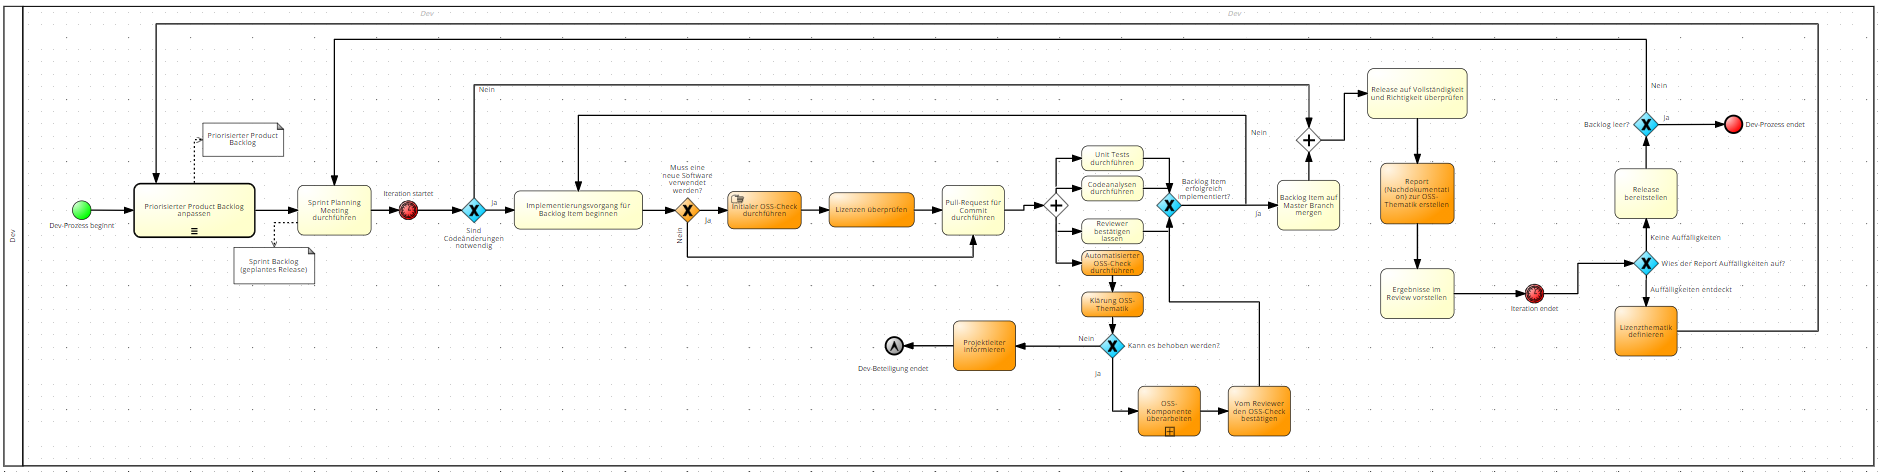
\includegraphics[angle=90, scale=0.7]{Bilder/SOLL-Prozess.png}
    \caption{Einbindung von OSS in den Softwareentwicklungsprozess basierend auf dem HAF-Projekt}
\end{figure}